\subsection{Architecture}
\subsubsection{Design Overview}
\textbf{VLANs} \\
The upgraded network ensures that departments and specific services are 
isolated (per the new network requirements) by distributing them across 
separate VLANs. This configuration allows for any combination of hosts assigned 
to different departments to be physically attached to the same switch (in the 
event that physical separation is not feasible), while maintaining separation.
\\

\noindent The VLANs are assigned as follows:
\newcolumntype{P}[1]{>{\centering\arraybackslash}p{#1}}
\setlength{\extrarowheight}{1ex}%
\renewcommand{\arraystretch}{1}%
\begin{center}
    \begin{tabular}{|P{2.0cm}|P{1.2cm}|P{4.0cm}|}
    \hline
        \textbf{Addresses} & \textbf{VLAN} & \textbf{Department/Service}\\
    \hline
        10.1.110.0/24 & 10 & Executives \\
    \hline
        10.1.120.0/24 & 20 & Human Resources \\
    \hline
        10.1.130.0/24 & 30 & Research \& Development \\
    \hline
        10.1.140.0/24 & 40 & Engineering \\
    \hline
        10.1.150.0/24 & 50 & Sales \\
    \hline
        10.1.160.0/24 & 60 & Internal Services \\
    \hline
        10.1.170.0/24 & 70 & DMZ \\
    \hline
\end{tabular}
\end{center}

\vspace{1em}

\noindent
\textbf{Inter-Router/Switch Interfaces} \\
Interfaces between router-router and switch-router (and vice versa) are assigned
addresses with a CIDR of /30. The address space \textbf{10.1.2.0/24} is reserved
specifically for these interfaces.  \\

\noindent
\textbf{Switch Ports} \\
Switch ports are statically assigned, as needed, within the address space of 
\textbf{10.1.10.0/24}. \\

\noindent
\textbf{Static Hosts} \\
Special hosts (specific services, such as DHCP, etc.) are assigned IP addresses 
statically within the address space of \textbf{10.1.160.0/24} for internal 
services, and within the address space of \textbf{10.1.170.0/24} for DMZ 
services. \\

\begin{center}
	\begin{tabular}[m]{| c | c |}
		\hline
		\multicolumn{2}{|c|}{Server Zone}\\
		\hline
		\textbf{Addresses} & \textbf{Service}\\
		\hline
		10.1.160.1 & DHCP \\
		\hline
		10.1.160.2 & DNS \\
		\hline
		10.1.160.3 & Active Directory \\
		\hline
		10.1.160.4 & Database \\
		\hline
		10.1.160.5 & NFS \\
		\hline
	\end{tabular}
\end{center}

\vspace{1em}


\begin{center}
	\begin{tabular}[m]{| c | c |}
		\hline
		\multicolumn{2}{|c|}{DMZ Zone}\\
		\hline
		\textbf{Addresses} & \textbf{Service}\\
		\hline
		10.1.170.1 & Web \\
		\hline
		10.1.170.2 & SMTP \\
		\hline
	\end{tabular}
\end{center}

\vspace{1em}

\noindent
\textbf{Workstation Hosts} \\
Workstation IP addresses are dynamically assigned by the DHCP server. 
Workstations are configured to use the IP of the switch port that that they are
physically connected to as their gateway to ensure that they connect to the 
network only via the preassigned switch port. \\

\subsubsection{Network Topology Map}
The upgraded Acme Corp. network is expanded from an all layer 2 network to a 
combination of layer 2 and layer 3 -- allowing for a more robust and "smart" 
network. The new network accounts for future expansion in the form of 
available ports on the four main routers that can host additional switches when
the time comes to expand the network. IP address availability is assured by
the spacing between VLAN subnets once the 254 useable addresses on a particular 
VLAN have been exhausted.
 
\begin{figure}[!htb]
	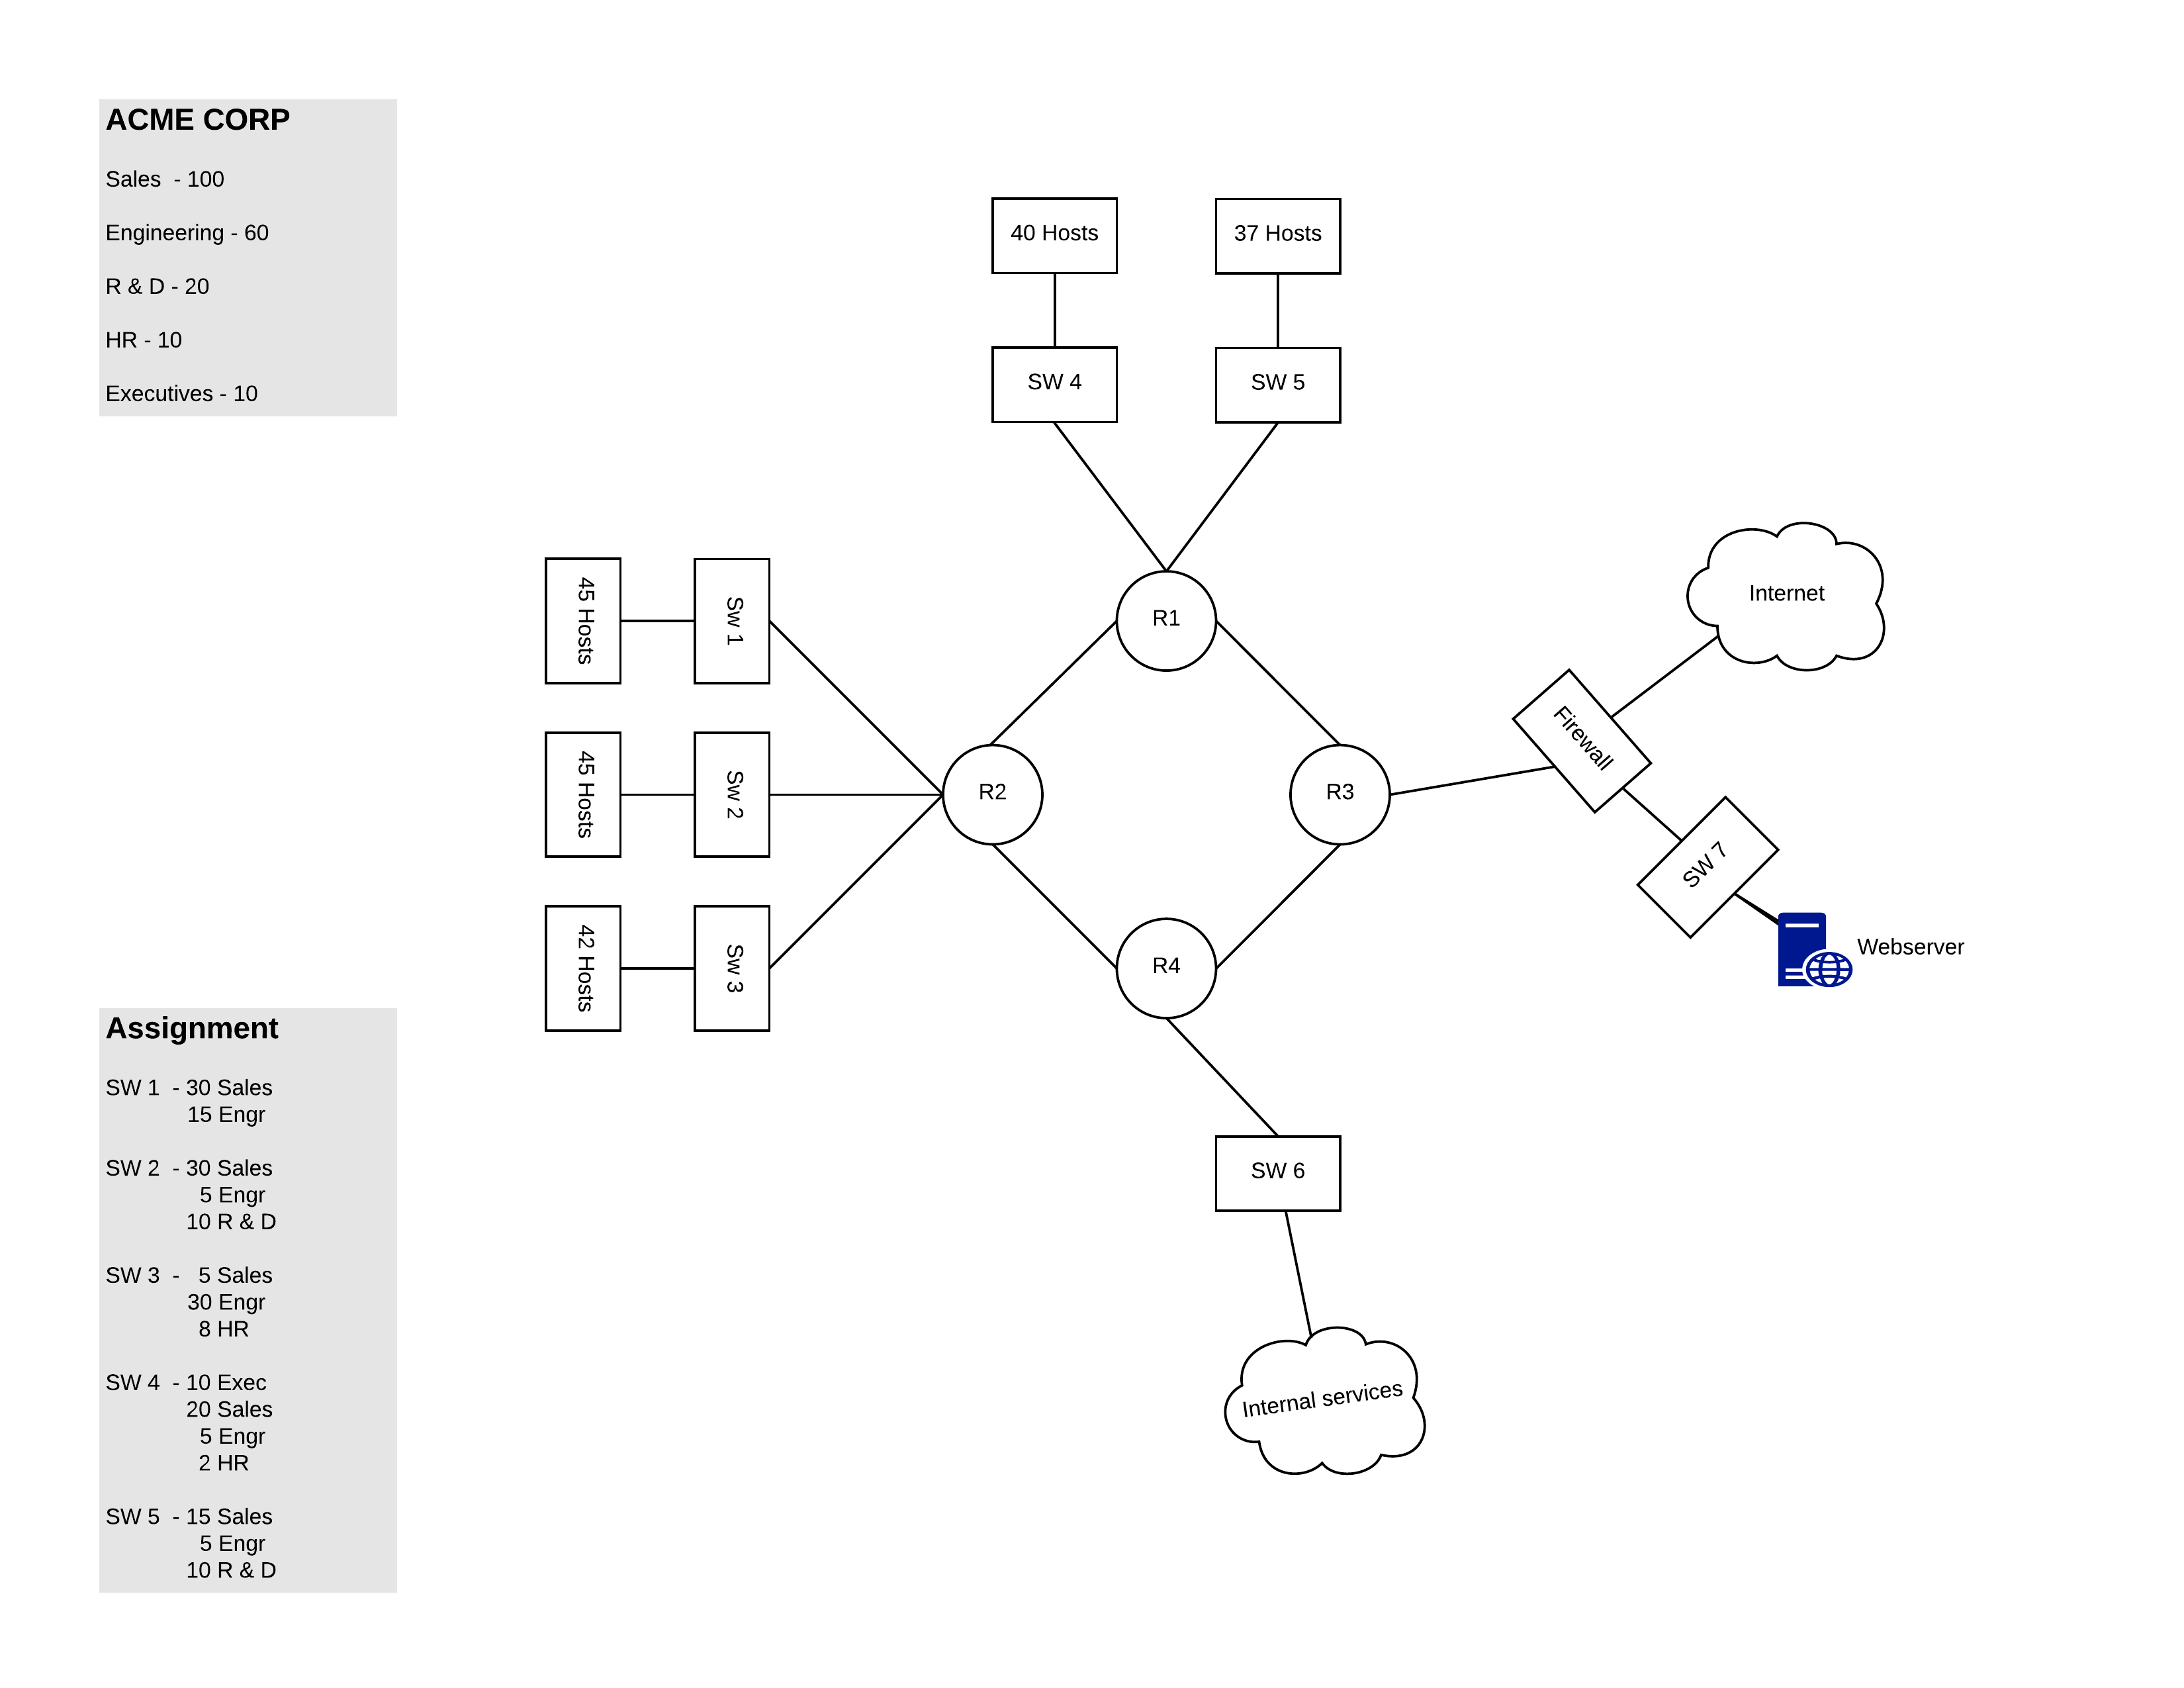
\includegraphics[width=\textwidth]{images/networktopology.png}
	\caption{Topology Map for Acme Corp}
\end{figure}
